\documentclass{article}
\PassOptionsToPackage{numbers}{natbib}
\usepackage[final]{neurips_2023}
\usepackage[utf8]{inputenc}
\usepackage[T1]{fontenc}
\usepackage{hyperref}
\usepackage{url}
\usepackage{booktabs}
\usepackage{amsmath}
\usepackage{amssymb}
\usepackage{graphicx}
\usepackage{xcolor}
\newcommand{\FID}{129.43}
\newcommand{\IS}{1.579}
\newcommand{\NumTrain}{3875}
\newcommand{\NumTest}{390}
\newcommand{\NumEpochs}{100}
\newcommand{\InitLoss}{2562.3}
\newcommand{\FinalLoss}{2403.1}
\newcommand{\MinLoss}{2402.2}
\newcommand{\MinLossEpoch}{97}
\newcommand{\Device}{RTX PRO 6000 Blackwell (1g.24gb MIG slice)}
\newcommand{\FIDRealRef}{20.5}
\newcommand{\FIDNoiseRef}{364.3}
\newcommand{\FIDSoftmax}{0.115}
\newcommand{\LossDropTenPct}{88}

\makeatletter\renewcommand{\@noticestring}{ECE 285, Homework 1 (Fall 2026).}\makeatother

\title{Generating Chest X-rays with a Convolutional Variational Autoencoder}

\author{%
  Oren Gershony \\
  ECE 285, Homework 1 \\
  \texttt{ogershony@gmail.com}
}

\begin{document}
\maketitle

\begin{abstract}
We implement a convolutional variational autoencoder (VAE)~\cite{kingma2014} in PyTorch and train it on the
pneumonia subset of the Kaggle chest X-ray dataset. We report hyperparameters, the loss curve,
Inception Score (IS) and Fr\'echet Inception Distance (FID) via PyTorch-Ignite, and samples. The model reaches an FID of \FID{} against
the test set (real held-out training images score \FIDRealRef{}, uniform noise \FIDNoiseRef{}) and an
IS of \IS{}.
\end{abstract}

\section{Setup}

\paragraph{Data.}
We use the chest X-ray pneumonia dataset~\cite{kermany2018}. The repository contains the
\textsc{Pneumonia} class only: \NumTrain{} training and \NumTest{} test images. Each image is
converted to a single grey channel, resized to $64{\times}64$ for compute reasons, and scaled to
$[0,1]$. No augmentation is used. All code (\texttt{VAE/}, \texttt{train.py}, \texttt{eval\_model.py},
\texttt{data.py}, \texttt{main.py}, \texttt{train\_gpu.sbatch}) is submitted with this report.

Table~\ref{tab:hparams} lists every setting; training ran on one NVIDIA \Device{} GPU.
Evaluation results are in Table~\ref{tab:metrics}.

\section{Results}

\paragraph{Training loss.}
Figure~\ref{fig:loss} shows the per-image training loss (reconstruction plus KL) over
\NumEpochs{} epochs. The loss falls from \InitLoss{} after the first epoch to \FinalLoss{} at
the end, with a minimum of \MinLoss{} at epoch \MinLossEpoch. About \LossDropTenPct\% of the decrease
happens in the first ten epochs; the loss is dominated by the reconstruction term.

\paragraph{Inception Score and FID.}
Following the PyTorch-Ignite recipe~\cite{ignite}, we decode one sample $z \sim \mathcal{N}(0, I)$
per real test image and update Ignite's \texttt{FID} and \texttt{InceptionScore} batch by batch.
Images are replicated to three channels and upsampled to $299{\times}299$ for the ImageNet
Inception-v3. FID uses the standard 2048-d pool features; Ignite's default \texttt{FID()} instead
uses the 1000-d softmax outputs, giving a meaningless \FIDSoftmax{} here, so we pass the
pool-feature extractor explicitly. For context, Table~\ref{tab:metrics} also scores \NumTest{} real
training images (\FIDRealRef, roughly the floor at this sample size) and uniform noise
(\FIDNoiseRef) against the test set. Our \FID{} lies about a third of the way from the real-data
floor to noise, consistent with the blurry samples. IS is close to its lower bound of 1 because
Inception assigns nearly the same class distribution to every chest X-ray, so FID is the more
informative metric.

\begin{table}[h]
  \centering
  \small
  \begin{minipage}[t]{0.52\textwidth}
    \centering
    \begin{tabular}{@{}ll@{}}
      \toprule
      Setting & Value \\
      \midrule
      Input & $64{\times}64$, 1 channel \\
      Latent dimension & 128 \\
      Optimiser & Adam, lr $10^{-3}$, default $\beta$ \\
      Batch size / epochs & 32 / \NumEpochs \\
      Loss & BCE (sum) $+$ KL, weight 1 \\
      Activations & LeakyReLU(0.2) enc., ReLU dec. \\
      Normalisation & BatchNorm \\
      Data loading & 8 workers, shuffled \\
      \bottomrule
    \end{tabular}
    \caption{Hyperparameters.}
    \label{tab:hparams}
  \end{minipage}\hfill
  \begin{minipage}[t]{0.45\textwidth}
    \centering
    \begin{tabular}{@{}lc@{}}
      \toprule
      Metric (vs.\ \NumTest{} test images) & Value \\
      \midrule
      FID $\downarrow$, VAE samples & \FID \\
      \quad real training images & \FIDRealRef \\
      \quad uniform noise & \FIDNoiseRef \\
      IS $\uparrow$, VAE samples & \IS \\
      \bottomrule
    \end{tabular}
    \caption{FID and IS (PyTorch-Ignite). Indented rows are reference points.}
    \label{tab:metrics}
  \end{minipage}
  \vspace{-8pt}
\end{table}

\begin{figure}[h]
  \centering
  \begin{minipage}[t]{0.46\textwidth}
    \centering
    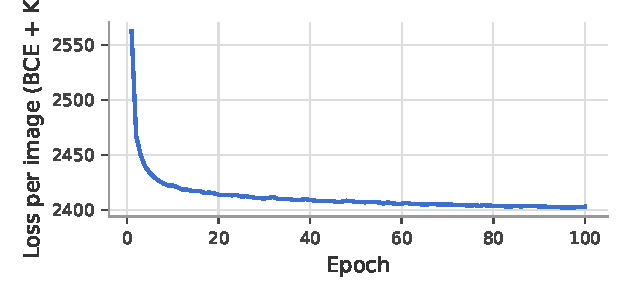
\includegraphics[width=\linewidth]{loss_curve.pdf}
    \caption{Training loss per image per epoch.}
    \label{fig:loss}
  \end{minipage}\hfill
  \begin{minipage}[t]{0.46\textwidth}
    \centering
    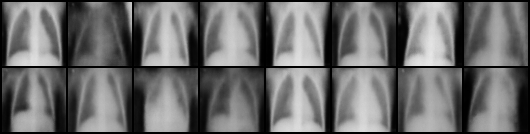
\includegraphics[width=\linewidth]{generated_grid.png}
    \caption{Sixteen samples decoded from $z \sim \mathcal{N}(0, I)$.}
    \label{fig:samples}
  \end{minipage}
  \vspace{-6pt}
\end{figure}

\paragraph{Generated images.}
Figure~\ref{fig:samples} shows sixteen random samples. The model captures the global anatomy
of a frontal chest radiograph: the dark lung fields, the bright mediastinum and spine, and the
shoulder and rib outline. As is typical of a VAE trained with a pixel-wise likelihood, the
samples are blurry and lack fine detail such as individual ribs or vessel markings. Higher
resolution, a perceptual reconstruction term, or a tempered KL weight are natural next steps.

\begin{thebibliography}{9}
\footnotesize
\bibitem{kingma2014} D.~P. Kingma and M. Welling. Auto-encoding variational Bayes. \emph{ICLR}, 2014.
\bibitem{kermany2018} D.~S. Kermany et al. Identifying medical diagnoses and treatable diseases by image-based deep learning. \emph{Cell}, 2018. \url{https://www.kaggle.com/paultimothymooney/chest-xray-pneumonia}.
\bibitem{ignite} PyTorch-Ignite. GAN evaluation with FID and IS. \url{https://pytorch-ignite.ai/blog/gan-evaluation-with-fid-and-is/}.
\end{thebibliography}

\end{document}
